The methodology for the research is based on the accessibilty of data
within our chosen network. Twitter, a popular platform for
Entrepreneurs and public discussion, has strong capabilities to propel
our research.

It was therefore decided to observe the public interactions of
Transnational Entrepreneurs on the Twitter network. Through Twitter's
public API we are able to get a host of publicly available data about
any given User, and their interactions within their egocentric network
(a network composed of a single individuals' friends and
followers). An abridged list of the possible data retrieved is as
follows:

\begin{itemize}
\item What is the user account description?
\item How many statuses has the User posted?
\item What is the time zone of the User?
\item Who are the friends of the User?
\item Who are the followers of the User?
\end{itemize}

\begin{figure}[!ht]
  \centering
  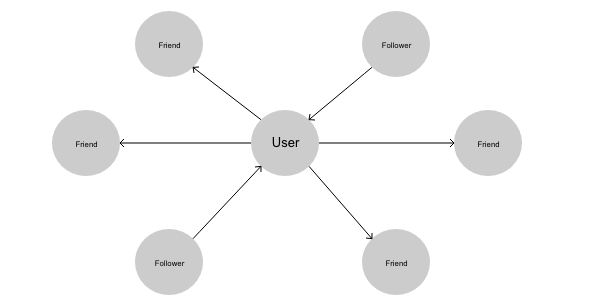
\includegraphics[width=1.0\textwidth]{egocentric.png}
  \caption{A simplified egocentric network.}
\end{figure}

\section{Cross-Sectional and Longitudinal}
All of this data allows us to reconstruct a Twitter User's activity,
and by extension, their network activity. Additionally important for
our research is: for any given user, Twitter, stores their last
200 Tweets.

The unique nature of the data on Twitter allows us to perform a mixed
longitudinal/cross-sectional approach. We examine several
Transnational Entrepreneurs within Berlin, and we examine their
network interactions for the duration of their last 200
Tweets. Depending on the activity of the user, this may span anywhere
from a day, to several years.

\section{Qualitative and Quantitative}
The research is mixed quantitative and qualitative analysis. This
capability is afforded to us by the Twitter public API which provides
deep data about users and their networks.

The quantitative research manifests itself in several ways. Firstly,
the Transnational Entreperneurs were selected quantitatively. Through
a series of filtering steps, they were identified. The filtering steps
relied on hard measures, such as, nationalityy distribution within
their ego centric network, or number of statuses tweeted.

After the identificaiton of the Transnational Entrepreneurs,
quantitative tools were then used in the analysis of their
networks. Automated quantitative analysis allowed the asking of
questions such as: How frequently were people in their network posting
about certain topics?  What were the dominant words used in their
interactions? Additionally, several network analysis measures were
assessed, in-betweeness-centrality, degree centrality, etc.

Finally, the qualitative analysis drew upon the results of the
quantitative studies. As an example, after collecting the egocentric
networks of Transnational Entrepreneurs, and creating word frequency
charts of their content, the charts were then analyzed from a
qualitative point of view. What are the individuals in the
Transnational Entrepreneur's networks talking about? How are they
related to each other? How do these conversations enhance the
Transnational Entrepreneur's ability to enterprise within their host
country?

\section{Inductive vs Deductive}
Deductive reasoning was chosen because of the characteristics of the
dataset that we have available to us. We first began with a testable
hypothesis - Transnational Diffusion frequency within a Transnational
Entrepreneur's egocentric network is moderated by their network's
country distribution.

Additionally important was the novelty of deductive reasoning within
this problem space. Prior research focused largely on case studies to
form broader generalizations (inductive), and we wanted to see if we
could validate/invalidate some of the generalized assumptions
discovered in inductive research.
